\section*{ARQUITECTURA DEL SISTEMA DE GESTIÓN DE CITAS MÉDICAS}
\begin{center}
\textit{Identificación de funciones, componentes, responsabilidades, relaciones, usuarios y base de datos}
\end{center}

\section{Identificación de las funciones principales}

A partir de la captura de requerimientos y de la especificación funcional, el sistema debe resolver las siguientes funciones principales:

\begin{itemize}
    \item Gestionar pacientes, médicos y sus datos básicos.
    \item Agendar citas y validar la disponibilidad del médico.
    \item Modificar, cancelar y controlar el estado de las citas.
    \item Registrar cobros y realizar el arqueo diario de caja.
    \item Controlar insumos, existencias, consumos y alertas de stock mínimo.
    \item Registrar compras, proveedores y facturas.
    \item Controlar medicamentos sujetos a prescripción médica.
    \item Generar reportes operativos, financieros, de productividad e inventario.
    \item Administrar usuarios, roles, permisos y auditoría.
\end{itemize}

\begin{figure}[htbp]
\centering
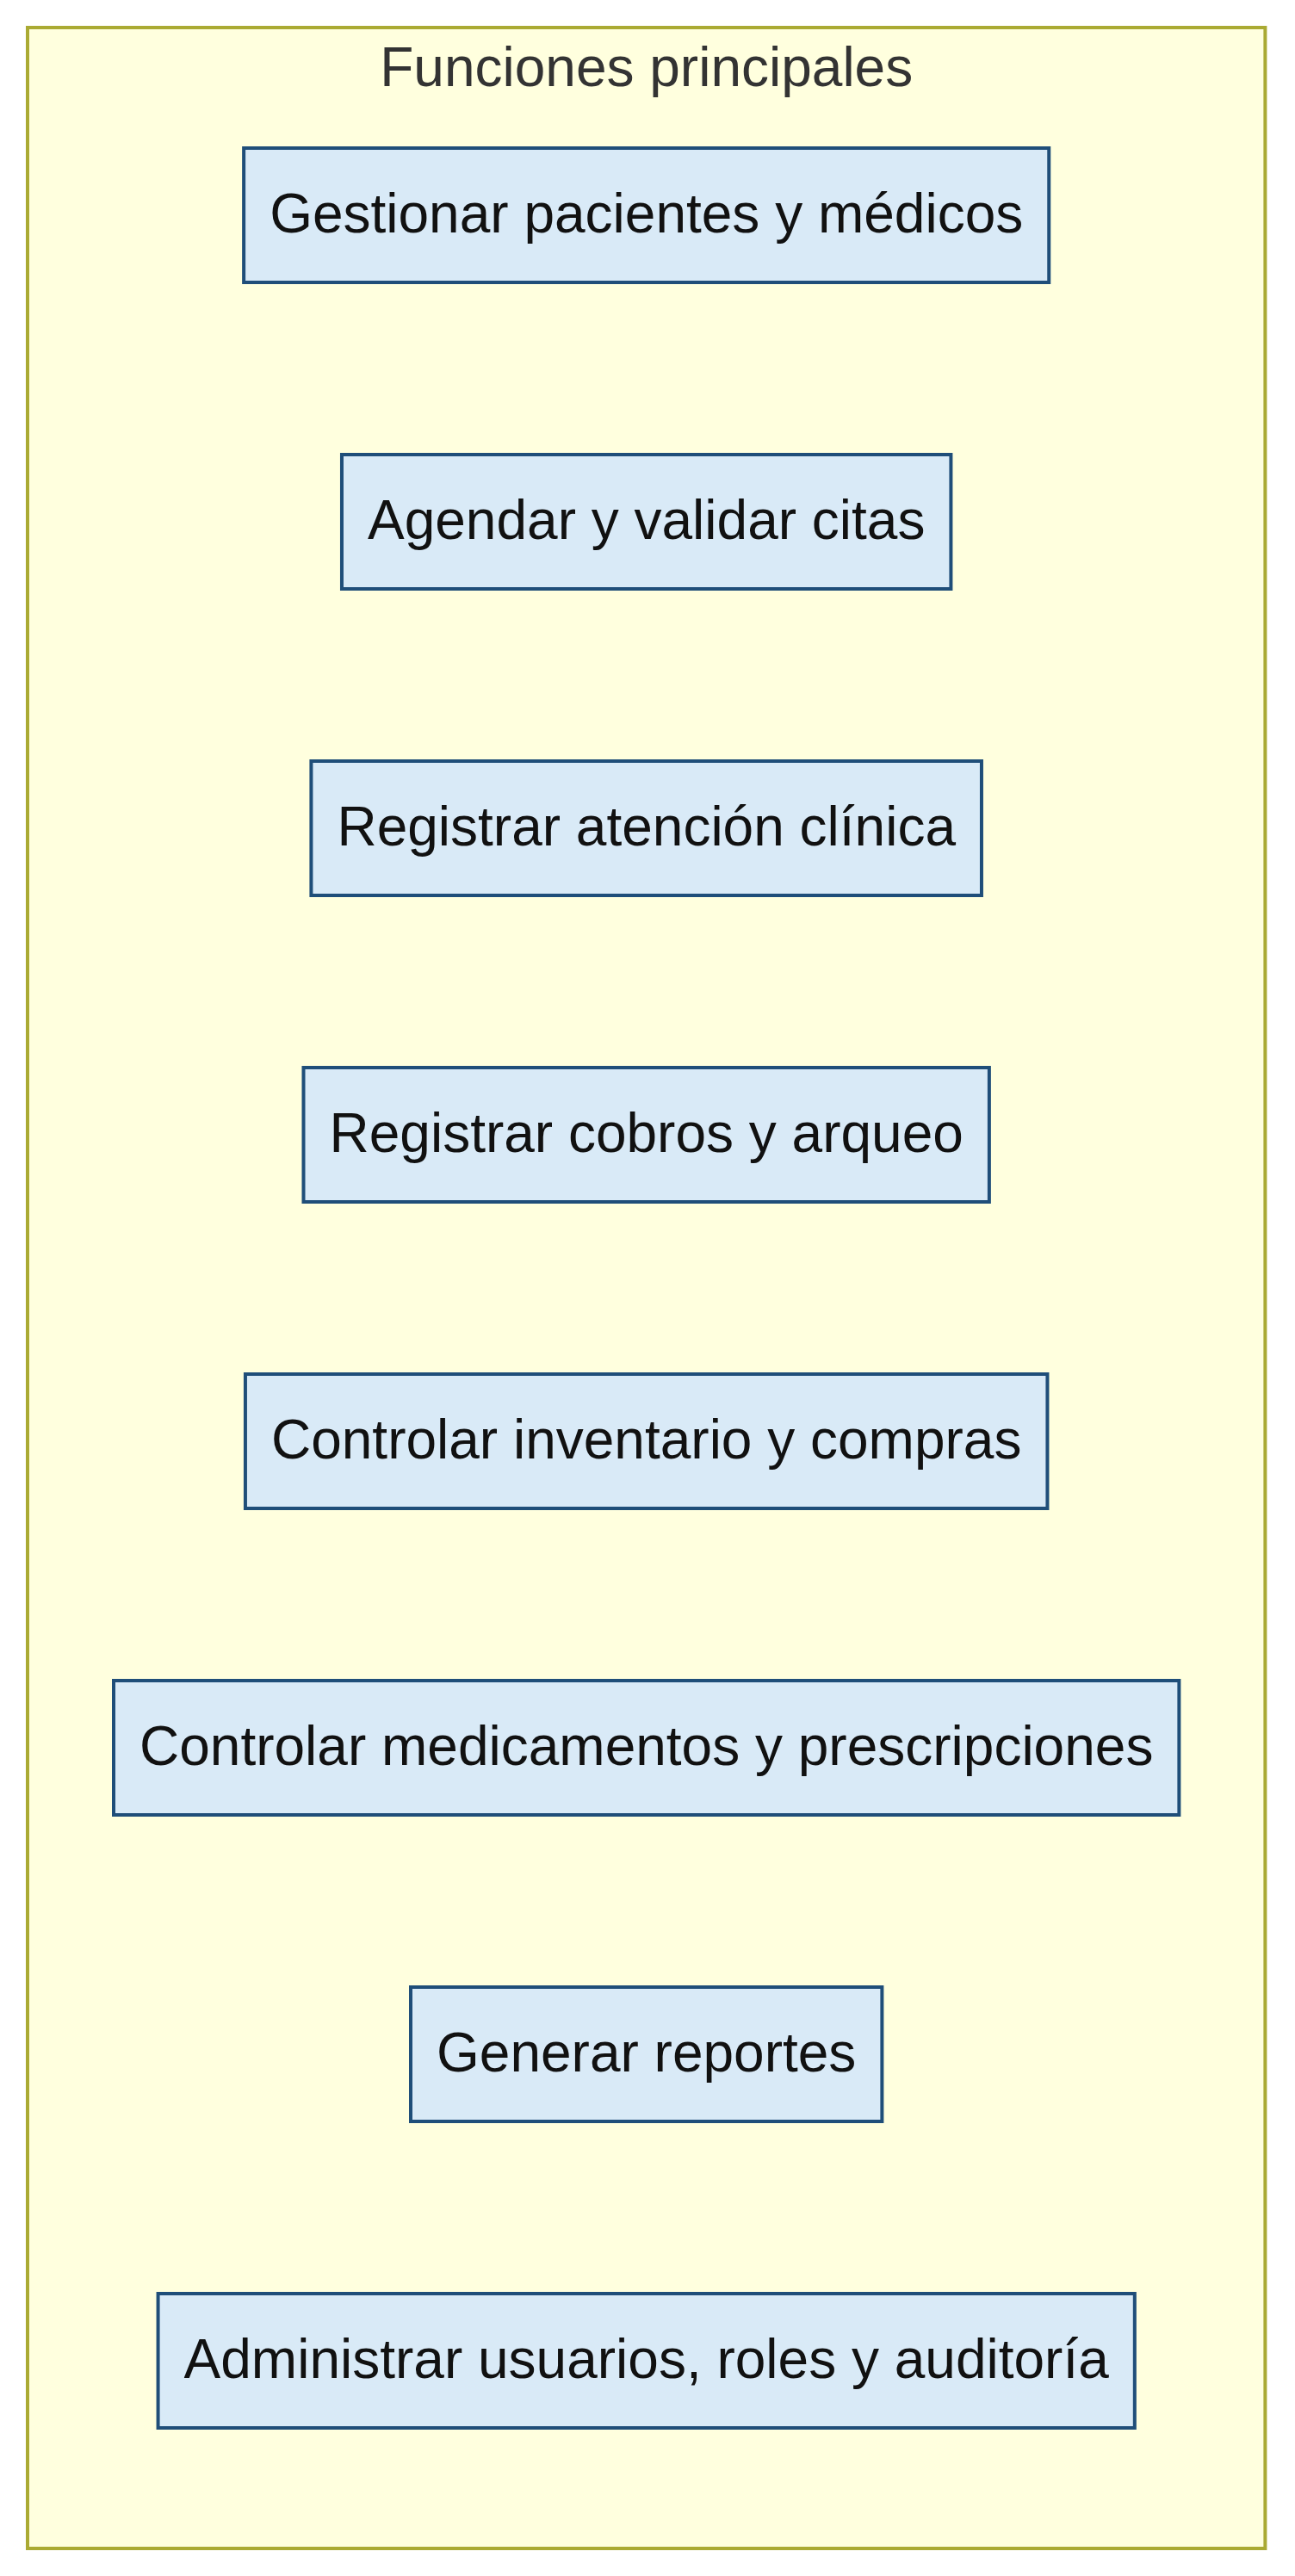
\includegraphics[width=\textwidth,height=0.52\textheight,keepaspectratio]{diagramas/draw1.png}
\caption{Funciones principales del sistema.}
\label{fig:funciones-principales}
\end{figure}

\section{Conversión de funciones en componentes}

Las funciones se agrupan en componentes cohesivos para separar responsabilidades y facilitar el mantenimiento del sistema. La agenda concentra las operaciones de citas; el componente clínico administra la atención y los consumos; y los componentes financiero, de inventario y de seguridad gestionan sus respectivos dominios.

\begin{figure}[htbp]
\centering
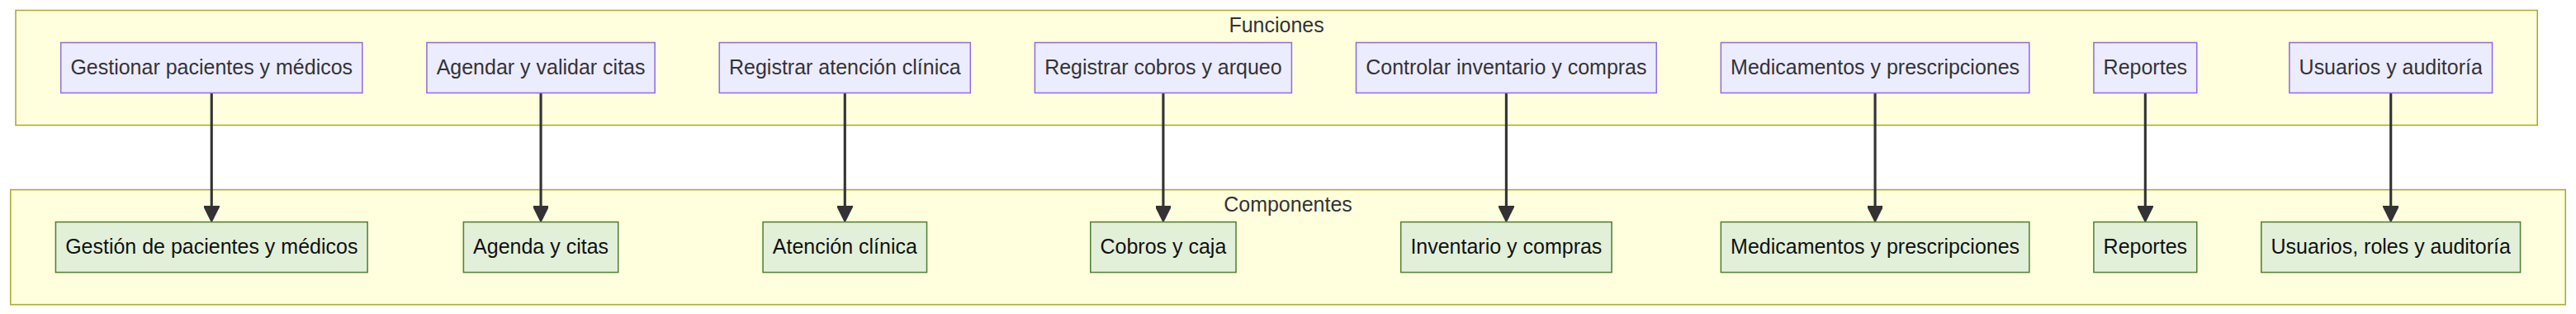
\includegraphics[width=\textwidth,height=0.52\textheight,keepaspectratio]{diagramas/draw2.png}
\caption{Correspondencia entre funciones y componentes del sistema.}
\label{fig:funciones-componentes}
\end{figure}

\section{Responsabilidades de los componentes}

La siguiente tabla establece qué información y operaciones administra cada componente identificado.

\small
\begin{tabularx}{\textwidth}{>{\bfseries}p{0.30\textwidth}X}
\toprule
\rowcolor{azulprincipal}\textcolor{white}{Componente} & \textcolor{white}{¿De qué se encarga?}\\
\midrule
Gestión de pacientes y médicos & Registrar y actualizar pacientes, médicos, especialidades, horarios y datos básicos necesarios para la atención.\\
Agenda y citas & Crear, consultar, modificar y cancelar citas; validar disponibilidad; controlar estados e historial de cambios.\\
Atención clínica & Registrar la atención, notas clínicas permitidas, prescripciones y consumos de insumos durante procedimientos.\\
Cobros y caja & Registrar montos, medios y estados de pago; generar el arqueo diario y bloquear modificaciones posteriores al cierre.\\
Inventario y compras & Administrar insumos, existencias, stock mínimo, entradas, salidas, consumos, proveedores y facturas.\\
Medicamentos y prescripciones & Vincular medicamentos sujetos a receta con el paciente, la consulta y la prescripción válida.\\
Reportes & Generar reportes de citas, cobros, compras, productividad médica e inventario con filtros por fecha.\\
Usuarios, roles y auditoría & Autenticar usuarios, autorizar operaciones según el rol y registrar usuario, fecha, hora y motivo de los cambios.\\
\bottomrule
\end{tabularx}
\normalsize

\begin{figure}[htbp]
\centering
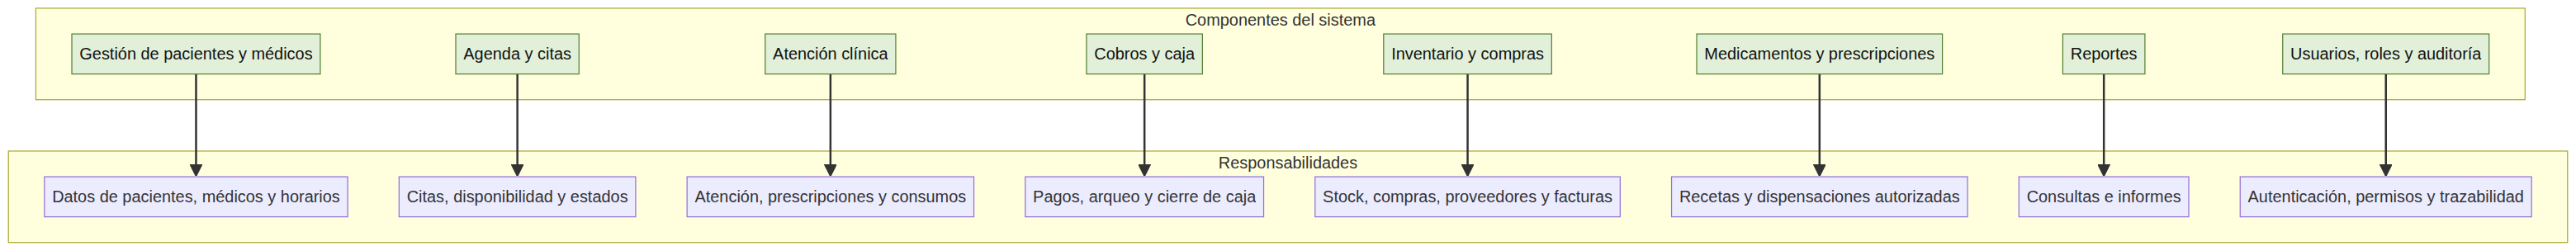
\includegraphics[width=\textwidth,height=0.52\textheight,keepaspectratio]{diagramas/draw3.png}
\caption{Componentes y responsabilidades principales.}
\label{fig:responsabilidades}
\end{figure}

\section{Relaciones entre componentes}

Las relaciones se definen mediante dependencias funcionales. La agenda utiliza pacientes y médicos para crear citas; la atención clínica consulta la agenda y descuenta los consumos del inventario; los cobros se relacionan con las citas; y los reportes consultan la información consolidada sin modificarla.

\begin{figure}[htbp]
\centering
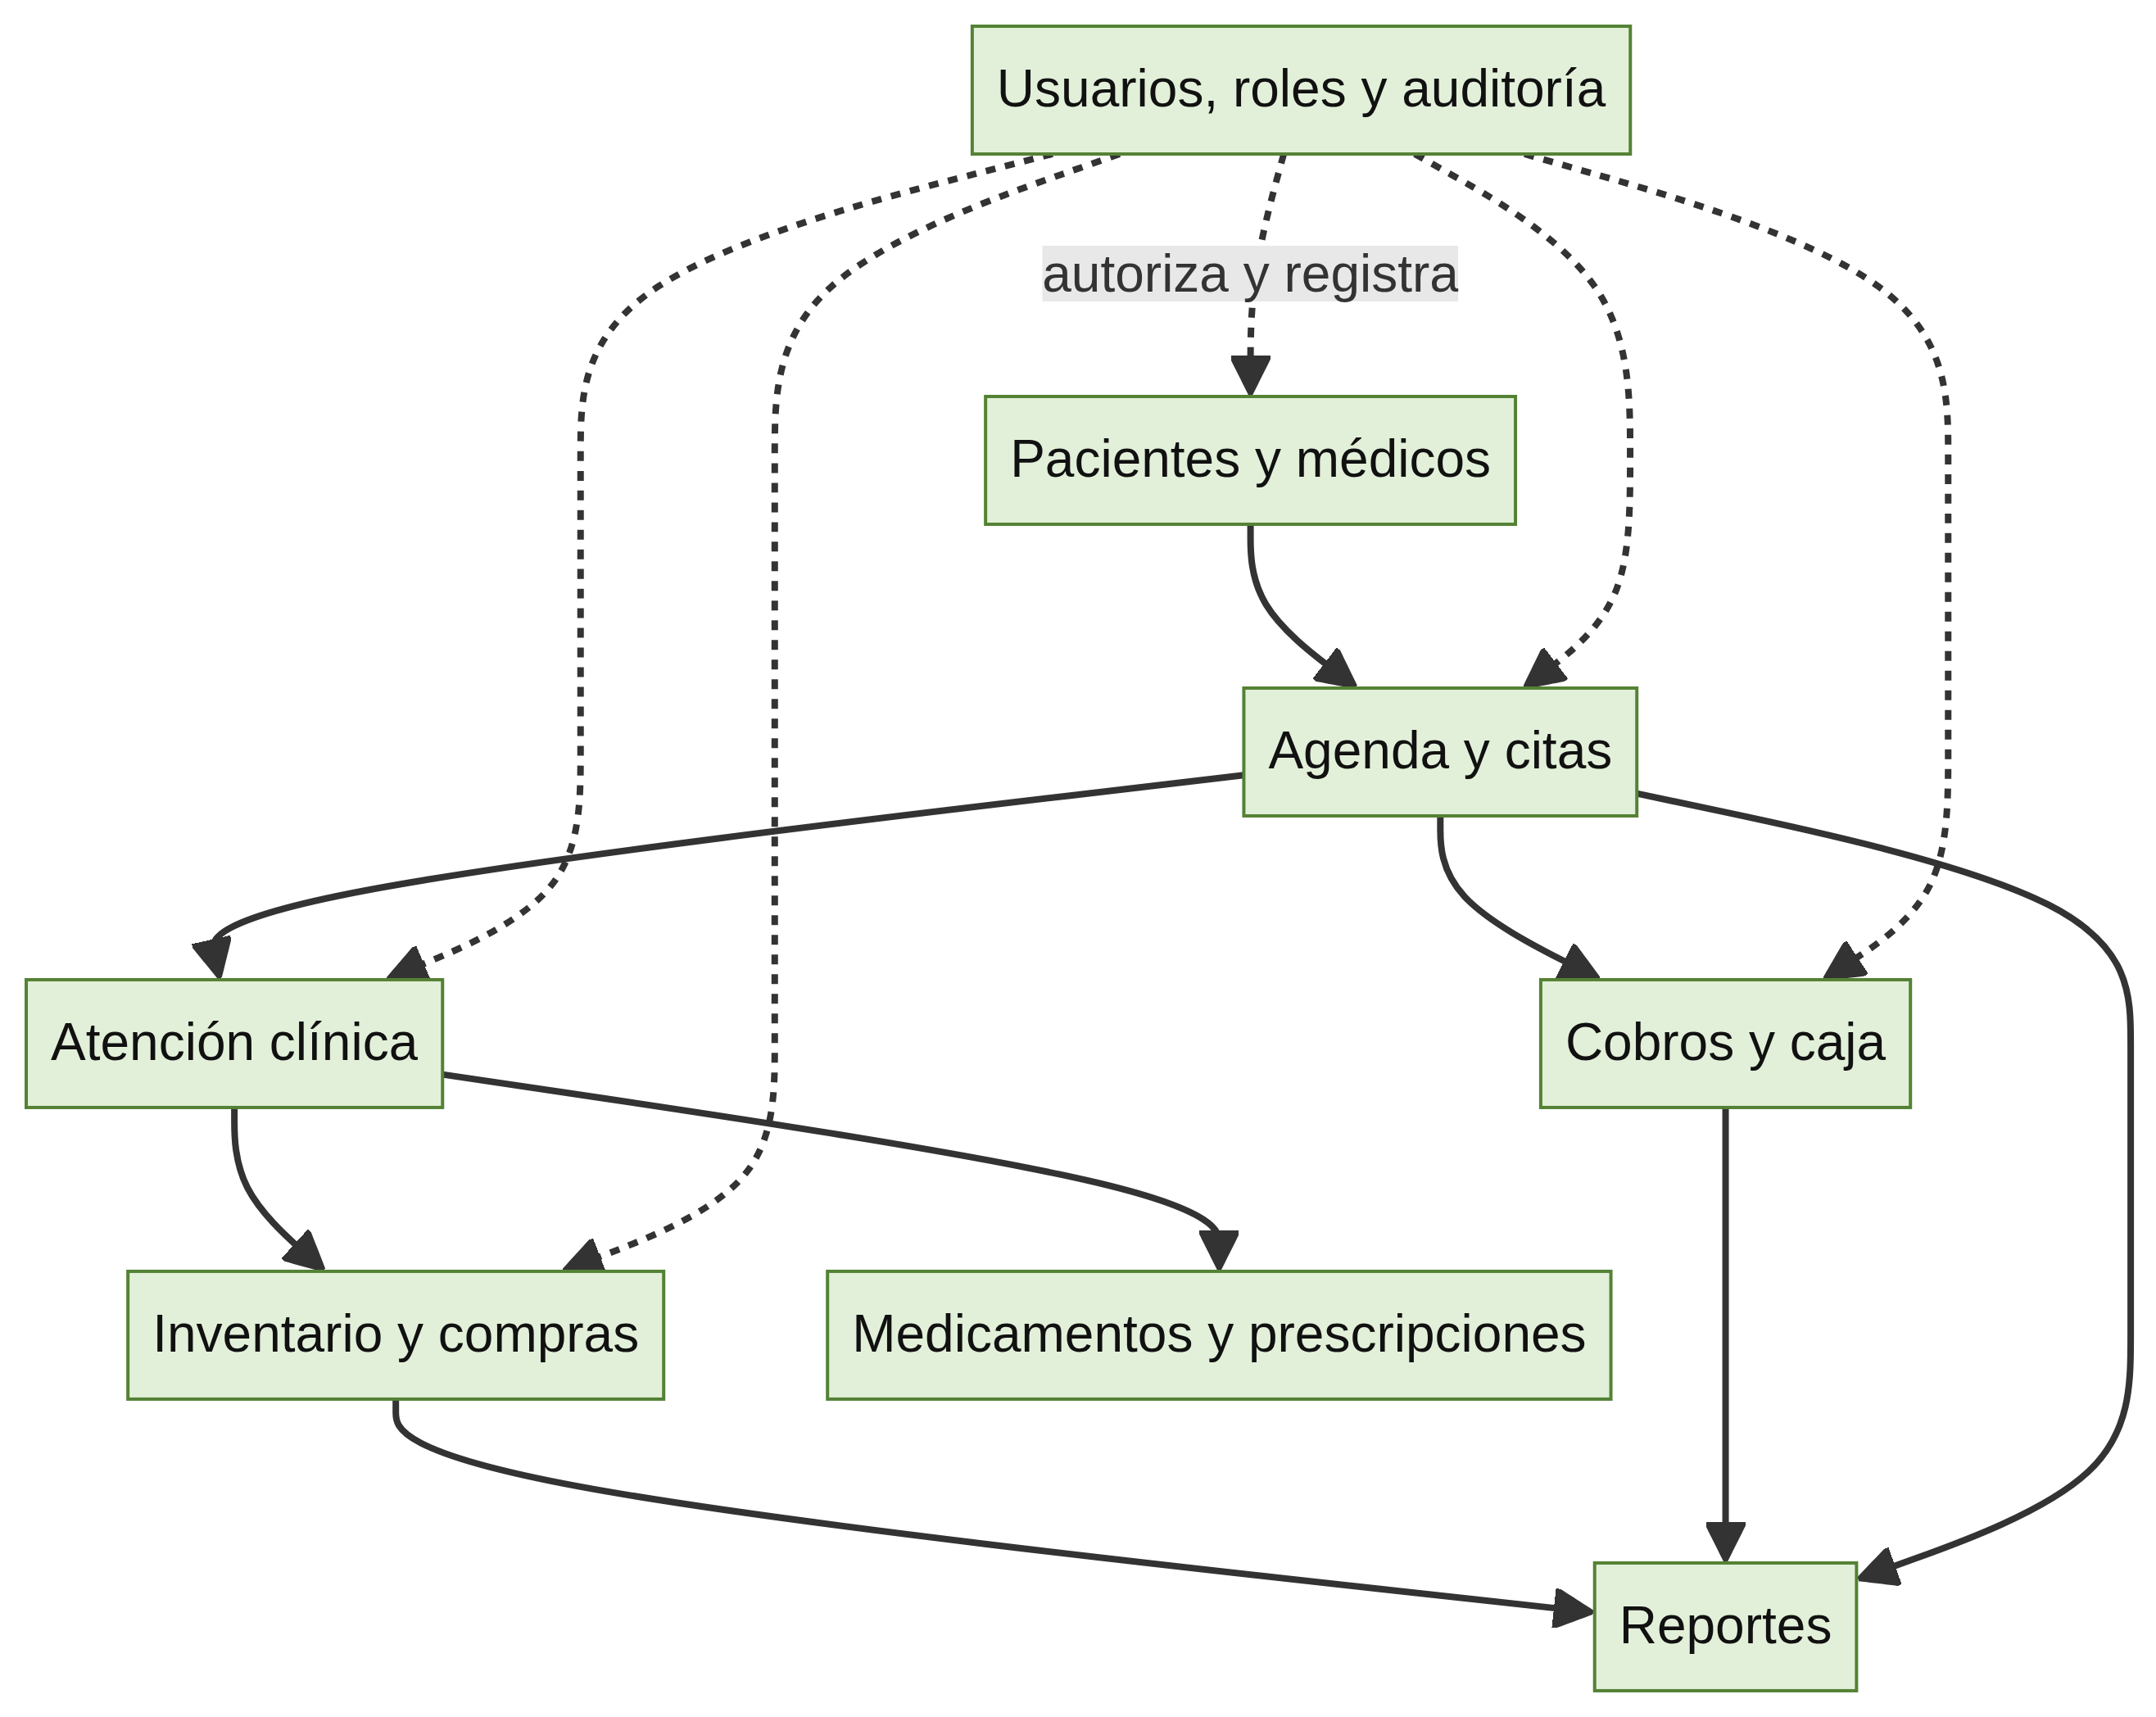
\includegraphics[width=\textwidth,height=0.52\textheight,keepaspectratio]{diagramas/draw4.png}
\caption{Relaciones y dependencias entre componentes.}
\label{fig:relaciones}
\end{figure}

\section{Usuarios del sistema}

Los usuarios y actores definidos en la captura de requerimientos interactúan con diferentes componentes según sus responsabilidades:

\begin{itemize}
    \item \textbf{Recepcionista:} registra pacientes, agenda citas, consulta disponibilidad, registra cobros y realiza el arqueo autorizado.
    \item \textbf{Médico:} consulta su agenda, registra la atención, emite prescripciones y declara los insumos consumidos.
    \item \textbf{Administrador:} administra usuarios, médicos, inventario, compras, parámetros y reportes.
    \item \textbf{Gerente general:} consulta información consolidada y reportes para supervisar la clínica.
    \item \textbf{Paciente:} proporciona sus datos, solicita citas y recibe confirmaciones o avisos.
\end{itemize}

\begin{figure}[htbp]
\centering
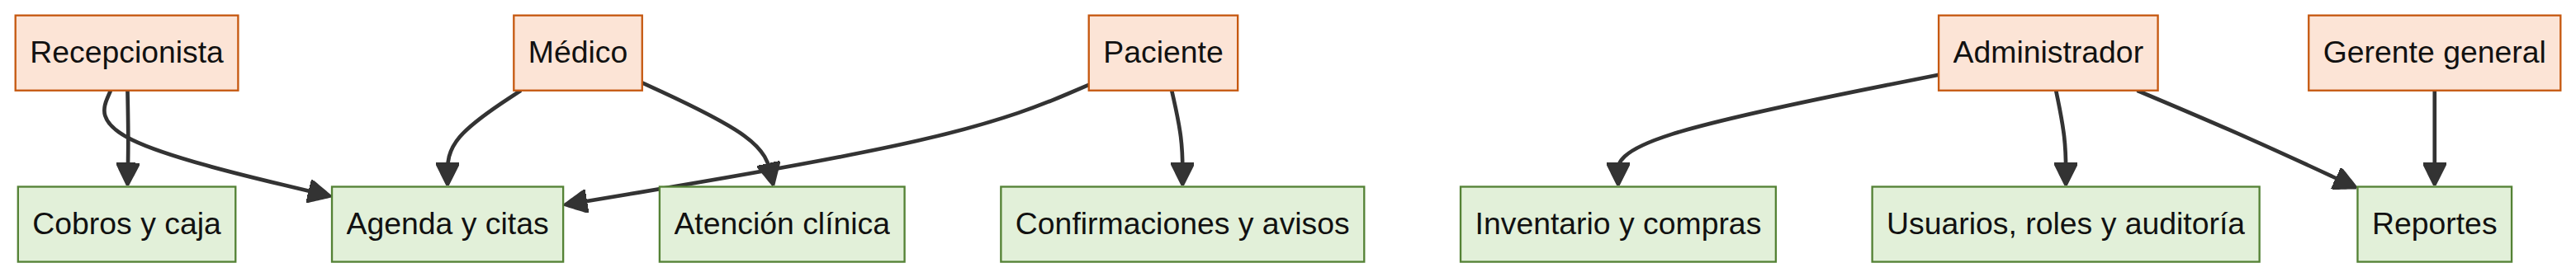
\includegraphics[width=\textwidth,height=0.52\textheight,keepaspectratio]{diagramas/draw5.png}
\caption{Usuarios y componentes con los que interactúan.}
\label{fig:usuarios}
\end{figure}

\section{Base de datos del sistema}

La base de datos debe centralizar la información y conservar la trazabilidad. Como mínimo, se identifican las entidades Paciente, Médico, Usuario, Cita, Atención, Prescripción, Medicamento, Insumo, Movimiento de inventario, Proveedor, Compra, Cobro y Auditoría. Las relaciones deben impedir citas solapadas, controlar existencias no negativas y vincular cobros y prescripciones con la atención correspondiente.

\begin{figure}[htbp]
\centering
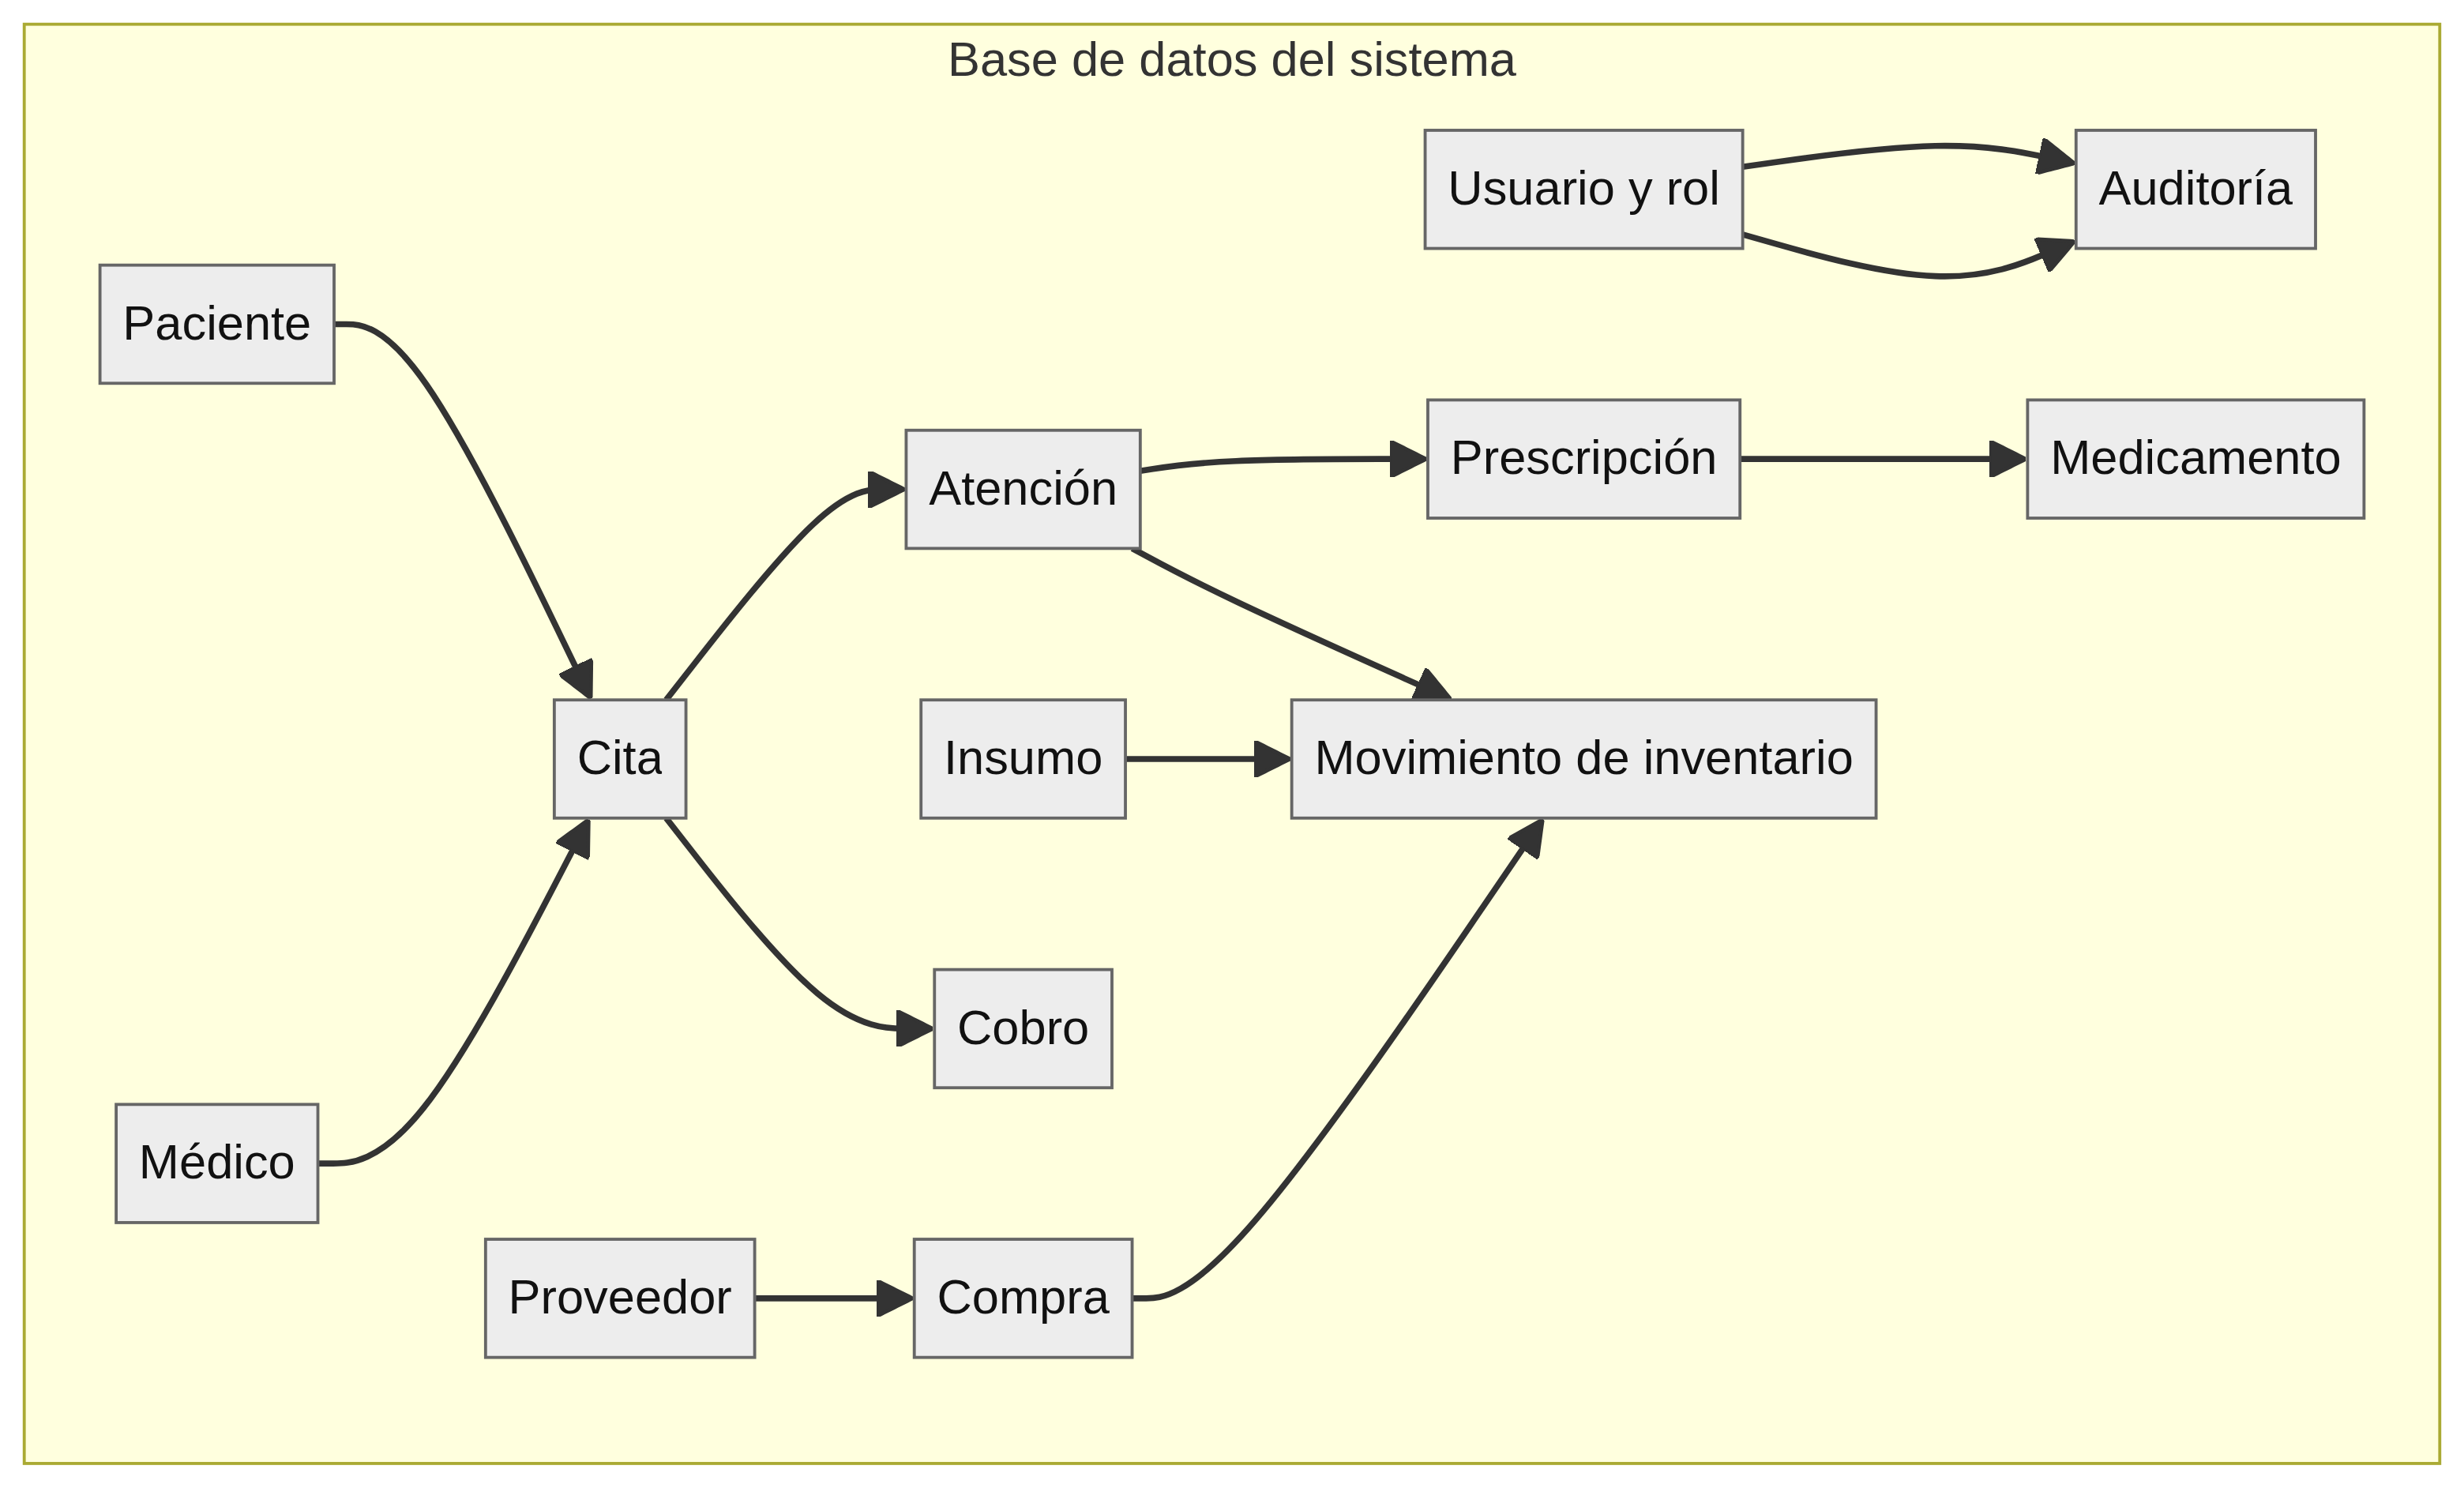
\includegraphics[width=\textwidth,height=0.52\textheight,keepaspectratio]{diagramas/draw6.png}
\caption{Base de datos conceptual y sus relaciones principales.}
\label{fig:base-datos}
\end{figure}

\section{Arquitectura del sistema}

Se propone una arquitectura por capas. La capa de presentación atiende las operaciones de los usuarios; la capa de aplicación coordina los casos de uso y aplica las reglas de negocio; la capa de dominio concentra las entidades y validaciones; y la capa de datos persiste la información. Los servicios transversales de autenticación, auditoría, reportes y respaldo apoyan a todas las capas.

Esta separación permite modificar la interfaz sin alterar las reglas de negocio, facilita las pruebas y protege la información clínica y administrativa mediante controles de acceso.

\begin{figure}[htbp]
\centering
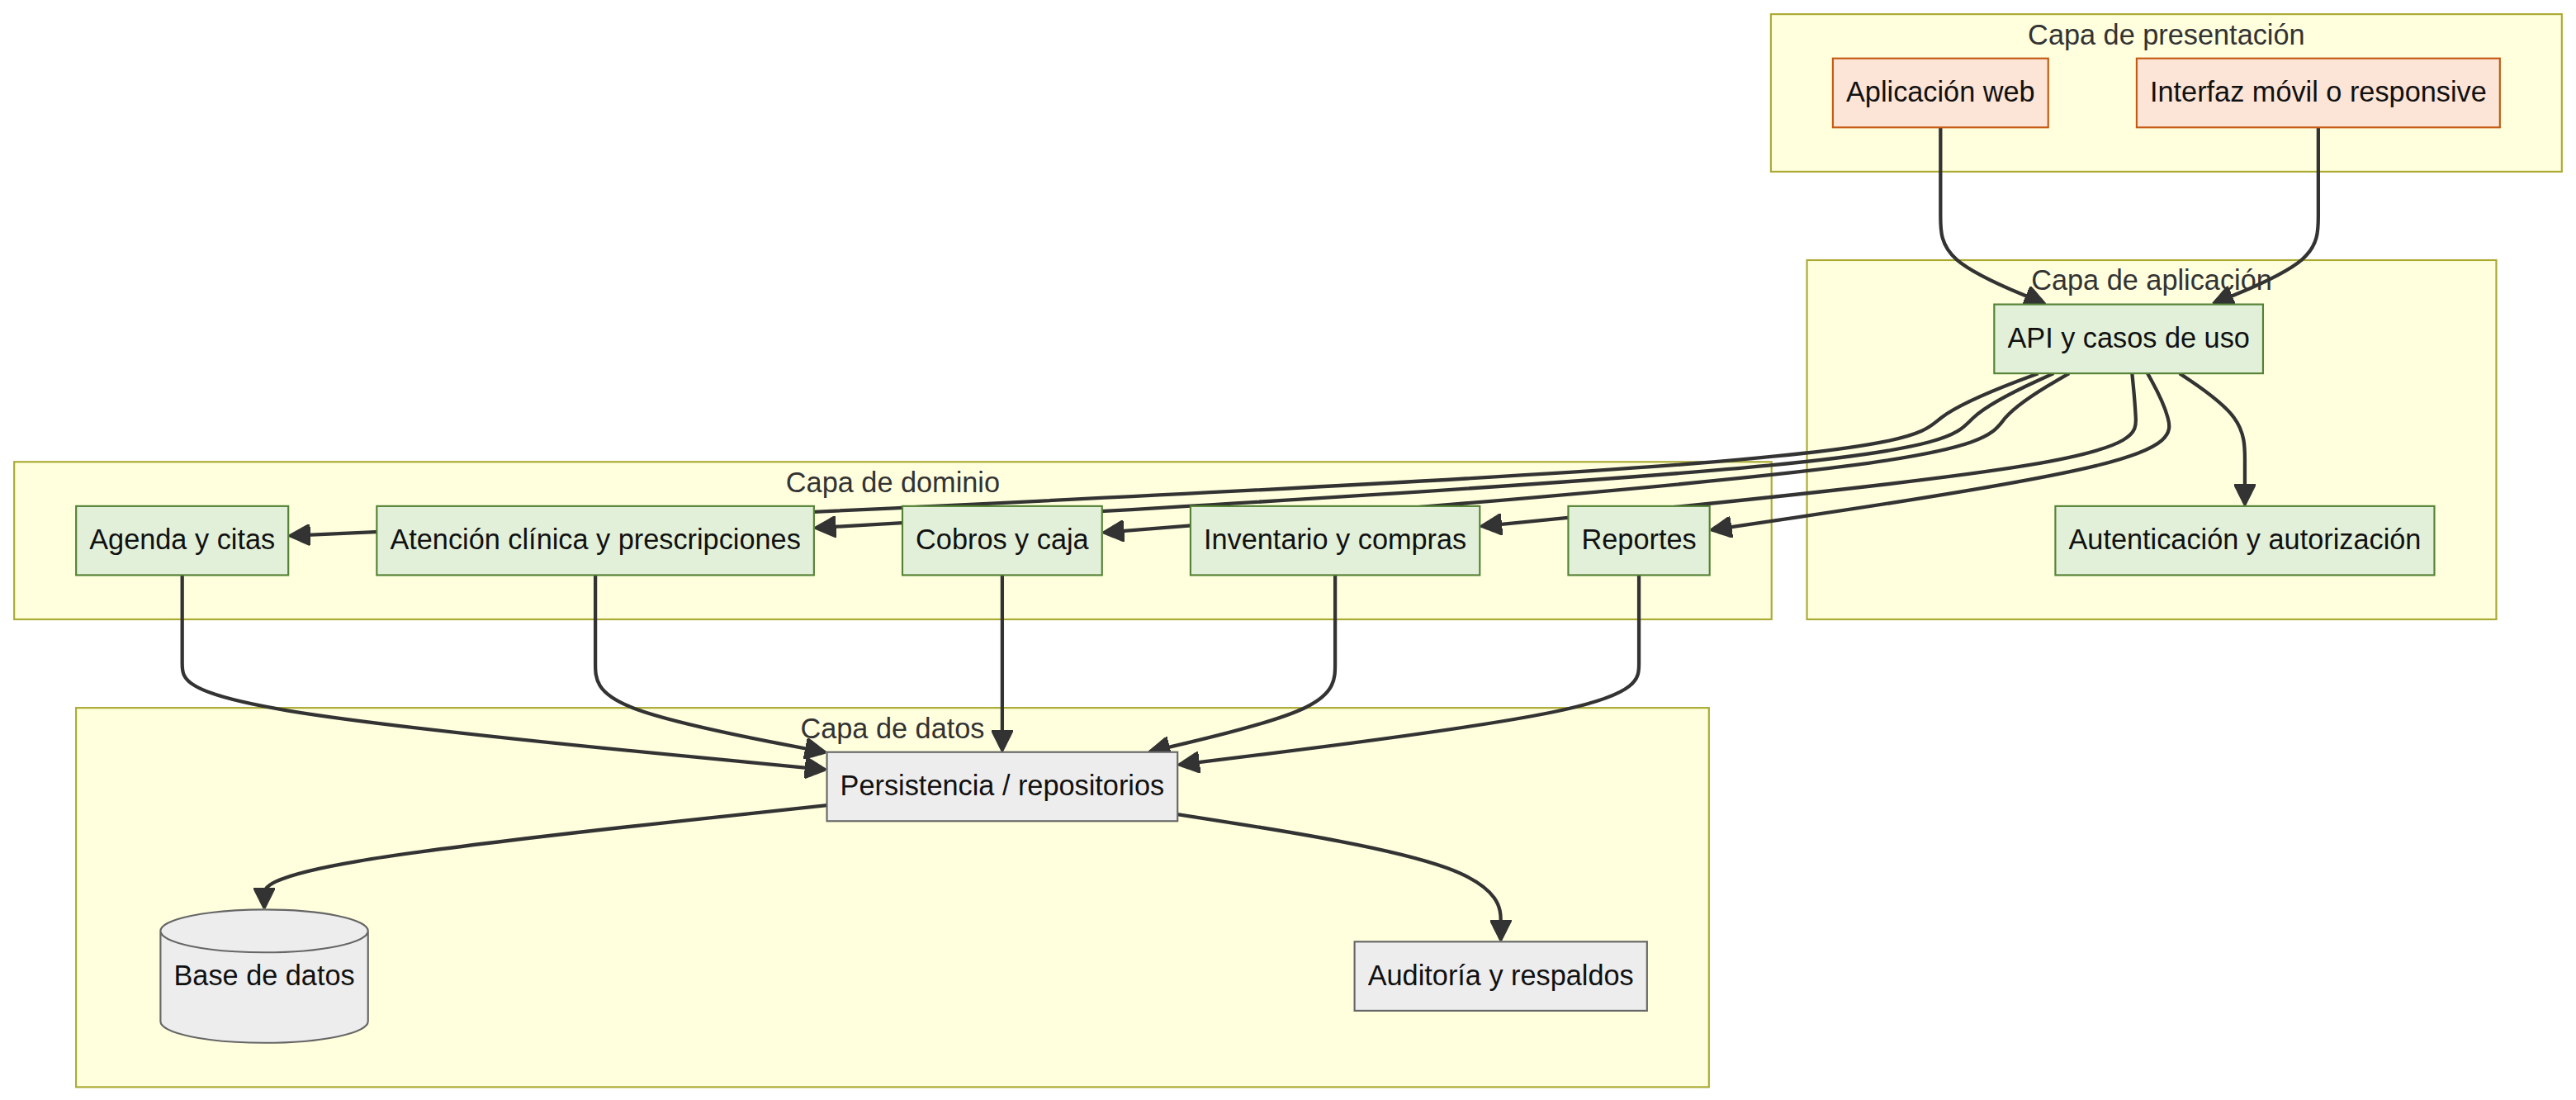
\includegraphics[width=\textwidth,height=0.52\textheight,keepaspectratio]{diagramas/draw7.png}
\caption{Arquitectura propuesta del sistema de gestión de citas médicas.}
\label{fig:arquitectura}
\end{figure}

\subsection*{Conclusión de la propuesta}

La solución transforma el proceso manual identificado en la entrevista en una arquitectura modular y trazable. Los componentes propuestos cubren las funciones prioritarias del proyecto, incorporan explícitamente a los usuarios y a la base de datos, y permiten implementar gradualmente la agenda, la atención clínica, los cobros, el inventario y los reportes.
